\documentclass[1p]{elsarticle_modified}
%\bibliographystyle{elsarticle-num}

%\usepackage[colorlinks]{hyperref}
%\usepackage{abbrmath_seonhwa} %\Abb, \Ascr, \Acal ,\Abf, \Afrak
\usepackage{amsfonts}
\usepackage{amssymb}
\usepackage{amsmath}
\usepackage{amsthm}
\usepackage{scalefnt}
\usepackage{amsbsy}
\usepackage{kotex}
\usepackage{caption}
\usepackage{subfig}
\usepackage{color}
\usepackage{graphicx}
\usepackage{xcolor} %% white, black, red, green, blue, cyan, magenta, yellow
\usepackage{float}
\usepackage{setspace}
\usepackage{hyperref}

\usepackage{tikz}
\usetikzlibrary{arrows}

\usepackage{multirow}
\usepackage{array} % fixed length table
\usepackage{hhline}

%%%%%%%%%%%%%%%%%%%%%
\makeatletter
\renewcommand*\env@matrix[1][\arraystretch]{%
	\edef\arraystretch{#1}%
	\hskip -\arraycolsep
	\let\@ifnextchar\new@ifnextchar
	\array{*\c@MaxMatrixCols c}}
\makeatother %https://tex.stackexchange.com/questions/14071/how-can-i-increase-the-line-spacing-in-a-matrix
%%%%%%%%%%%%%%%

\usepackage[normalem]{ulem}

\newcommand{\msout}[1]{\ifmmode\text{\sout{\ensuremath{#1}}}\else\sout{#1}\fi}
%SOURCE: \msout is \stkout macro in https://tex.stackexchange.com/questions/20609/strikeout-in-math-mode

\newcommand{\cancel}[1]{
	\ifmmode
	{\color{red}\msout{#1}}
	\else
	{\color{red}\sout{#1}}
	\fi
}

\newcommand{\add}[1]{
	{\color{blue}\uwave{#1}}
}

\newcommand{\replace}[2]{
	\ifmmode
	{\color{red}\msout{#1}}{\color{blue}\uwave{#2}}
	\else
	{\color{red}\sout{#1}}{\color{blue}\uwave{#2}}
	\fi
}

\newcommand{\Sol}{\mathcal{S}} %segment
\newcommand{\D}{D} %diagram
\newcommand{\A}{\mathcal{A}} %arc


%%%%%%%%%%%%%%%%%%%%%%%%%%%%%5 test

\def\sl{\operatorname{\textup{SL}}(2,\Cbb)}
\def\psl{\operatorname{\textup{PSL}}(2,\Cbb)}
\def\quan{\mkern 1mu \triangleright \mkern 1mu}

\theoremstyle{definition}
\newtheorem{thm}{Theorem}[section]
\newtheorem{prop}[thm]{Proposition}
\newtheorem{lem}[thm]{Lemma}
\newtheorem{ques}[thm]{Question}
\newtheorem{cor}[thm]{Corollary}
\newtheorem{defn}[thm]{Definition}
\newtheorem{exam}[thm]{Example}
\newtheorem{rmk}[thm]{Remark}
\newtheorem{alg}[thm]{Algorithm}

\newcommand{\I}{\sqrt{-1}}
\begin{document}

%\begin{frontmatter}
%
%\title{Boundary parabolic representations of knots up to 8 crossings}
%
%%% Group authors per affiliation:
%\author{Yunhi Cho} 
%\address{Department of Mathematics, University of Seoul, Seoul, Korea}
%\ead{yhcho@uos.ac.kr}
%
%
%\author{Seonhwa Kim} %\fnref{s_kim}}
%\address{Center for Geometry and Physics, Institute for Basic Science, Pohang, 37673, Korea}
%\ead{ryeona17@ibs.re.kr}
%
%\author{Hyuk Kim}
%\address{Department of Mathematical Sciences, Seoul National University, Seoul 08826, Korea}
%\ead{hyukkim@snu.ac.kr}
%
%\author{Seokbeom Yoon}
%\address{Department of Mathematical Sciences, Seoul National University, Seoul, 08826,  Korea}
%\ead{sbyoon15@snu.ac.kr}
%
%\begin{abstract}
%We find all boundary parabolic representation of knots up to 8 crossings.
%
%\end{abstract}
%\begin{keyword}
%    \MSC[2010] 57M25 
%\end{keyword}
%
%\end{frontmatter}

%\linenumbers
%\tableofcontents
%
\newcommand\colored[1]{\textcolor{white}{\rule[-0.35ex]{0.8em}{1.4ex}}\kern-0.8em\color{red} #1}%
%\newcommand\colored[1]{\textcolor{white}{ #1}\kern-2.17ex	\textcolor{white}{ #1}\kern-1.81ex	\textcolor{white}{ #1}\kern-2.15ex\color{red}#1	}

{\Large $\underline{12a_{0734}~(K12a_{0734})}$}

\setlength{\tabcolsep}{10pt}
\renewcommand{\arraystretch}{1.6}
\vspace{1cm}\begin{tabular}{m{100pt}>{\centering\arraybackslash}m{274pt}}
\multirow{5}{120pt}{
	\centering
	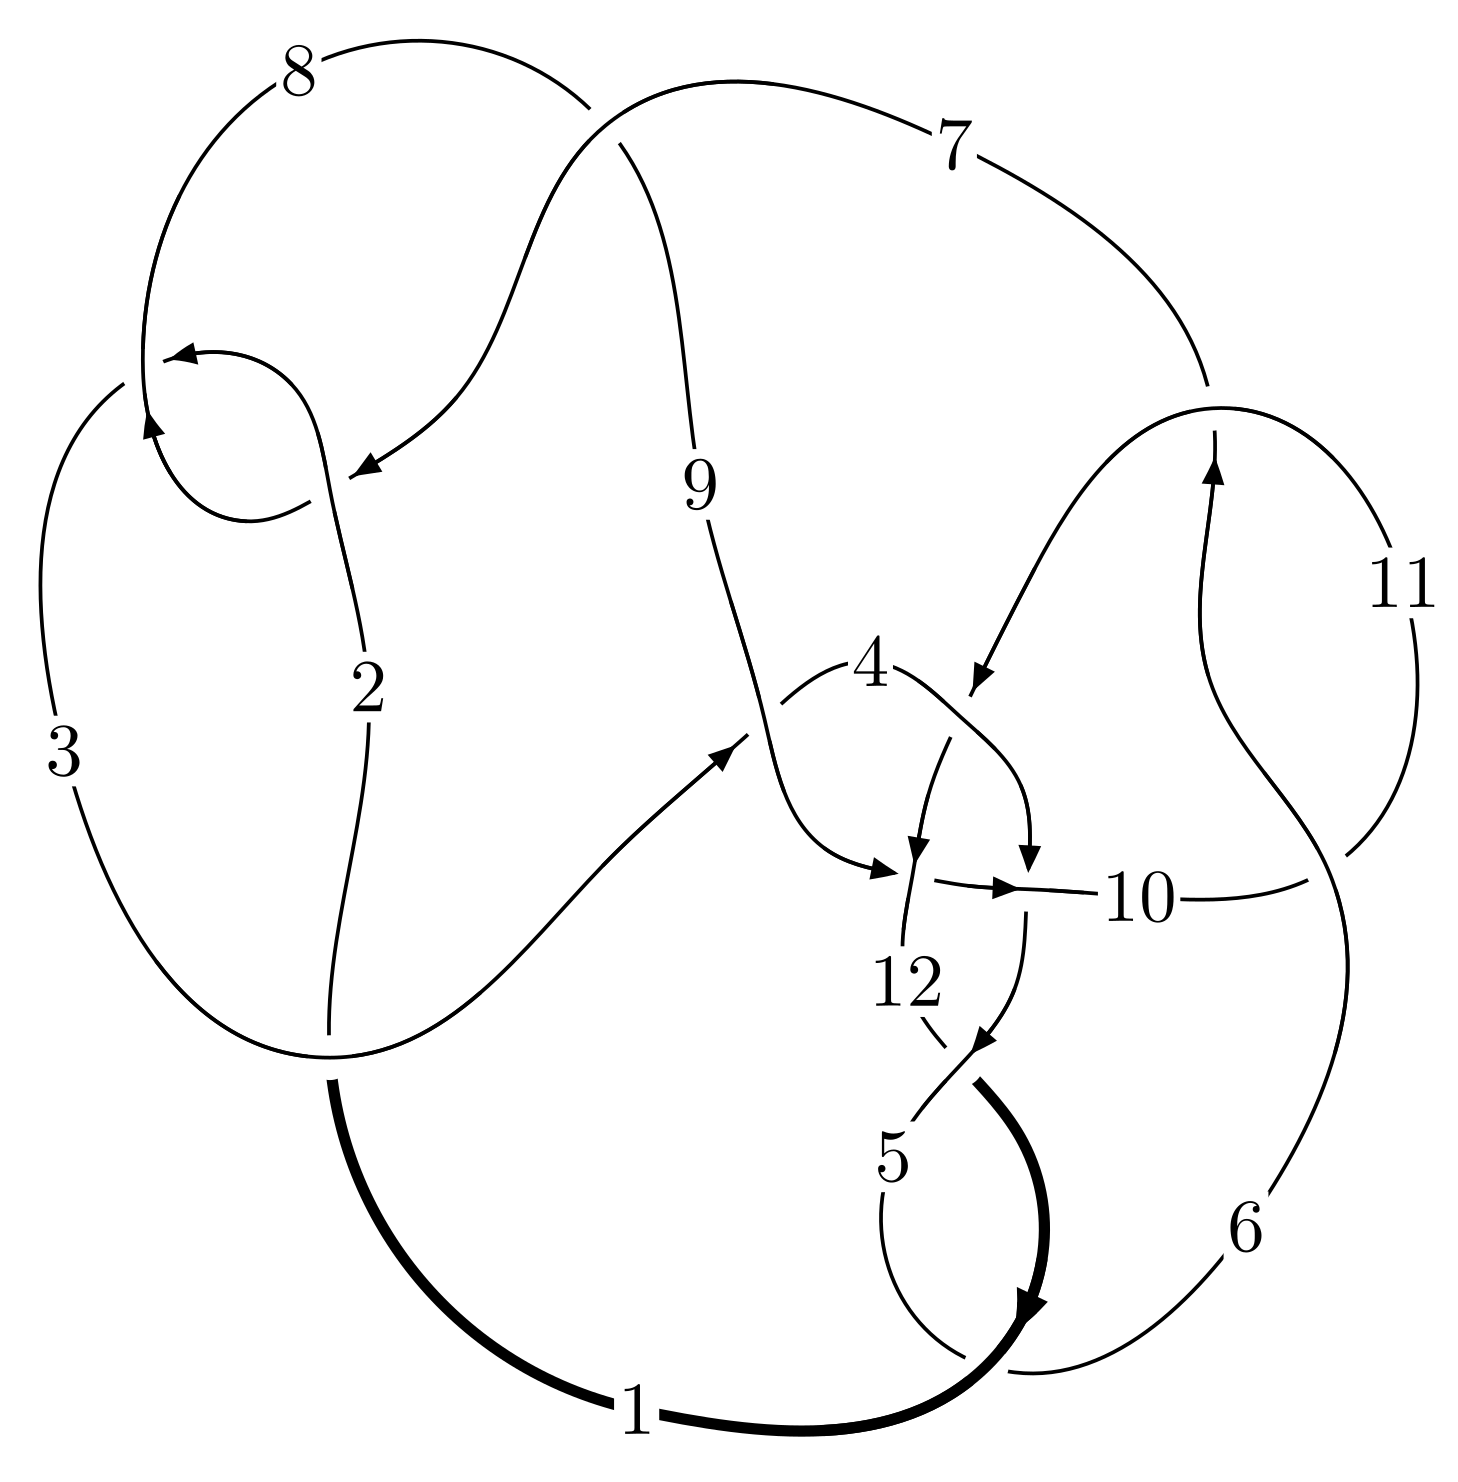
\includegraphics[width=112pt]{../../../GIT/diagram.site/Diagrams/png/1535_12a_0734.png}\\
\ \ \ A knot diagram\footnotemark}&
\allowdisplaybreaks
\textbf{Linearized knot diagam} \\
\cline{2-2}
 &
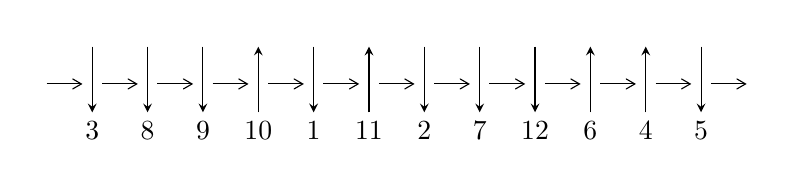
\begin{tikzpicture}[x=20pt, y=17pt]
	% nodes
	\node (C0) at (0, 0) {};
	\node (C1) at (1, 0) {};
	\node (C1U) at (1, +1) {};
	\node (C1D) at (1, -1) {3};

	\node (C2) at (2, 0) {};
	\node (C2U) at (2, +1) {};
	\node (C2D) at (2, -1) {8};

	\node (C3) at (3, 0) {};
	\node (C3U) at (3, +1) {};
	\node (C3D) at (3, -1) {9};

	\node (C4) at (4, 0) {};
	\node (C4U) at (4, +1) {};
	\node (C4D) at (4, -1) {10};

	\node (C5) at (5, 0) {};
	\node (C5U) at (5, +1) {};
	\node (C5D) at (5, -1) {1};

	\node (C6) at (6, 0) {};
	\node (C6U) at (6, +1) {};
	\node (C6D) at (6, -1) {11};

	\node (C7) at (7, 0) {};
	\node (C7U) at (7, +1) {};
	\node (C7D) at (7, -1) {2};

	\node (C8) at (8, 0) {};
	\node (C8U) at (8, +1) {};
	\node (C8D) at (8, -1) {7};

	\node (C9) at (9, 0) {};
	\node (C9U) at (9, +1) {};
	\node (C9D) at (9, -1) {12};

	\node (C10) at (10, 0) {};
	\node (C10U) at (10, +1) {};
	\node (C10D) at (10, -1) {6};

	\node (C11) at (11, 0) {};
	\node (C11U) at (11, +1) {};
	\node (C11D) at (11, -1) {4};

	\node (C12) at (12, 0) {};
	\node (C12U) at (12, +1) {};
	\node (C12D) at (12, -1) {5};
	\node (C13) at (13, 0) {};

	% arrows
	\draw[->,>={angle 60}]
	(C0) edge (C1) (C1) edge (C2) (C2) edge (C3) (C3) edge (C4) (C4) edge (C5) (C5) edge (C6) (C6) edge (C7) (C7) edge (C8) (C8) edge (C9) (C9) edge (C10) (C10) edge (C11) (C11) edge (C12) (C12) edge (C13) ;	\draw[->,>=stealth]
	(C1U) edge (C1D) (C2U) edge (C2D) (C3U) edge (C3D) (C4D) edge (C4U) (C5U) edge (C5D) (C6D) edge (C6U) (C7U) edge (C7D) (C8U) edge (C8D) (C9U) edge (C9D) (C10D) edge (C10U) (C11D) edge (C11U) (C12U) edge (C12D) ;
	\end{tikzpicture} \\
\hhline{~~} \\& 
\textbf{Solving Sequence} \\ \cline{2-2} 
 &
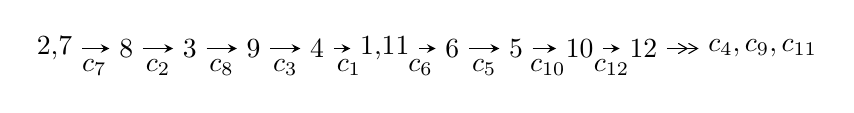
\begin{tikzpicture}[x=23pt, y=7pt]
	% node
	\node (A0) at (-1/8, 0) {2,7};
	\node (A1) at (1, 0) {8};
	\node (A2) at (2, 0) {3};
	\node (A3) at (3, 0) {9};
	\node (A4) at (4, 0) {4};
	\node (A5) at (81/16, 0) {1,11};
	\node (A6) at (49/8, 0) {6};
	\node (A7) at (57/8, 0) {5};
	\node (A8) at (65/8, 0) {10};
	\node (A9) at (73/8, 0) {12};
	\node (C1) at (1/2, -1) {$c_{7}$};
	\node (C2) at (3/2, -1) {$c_{2}$};
	\node (C3) at (5/2, -1) {$c_{8}$};
	\node (C4) at (7/2, -1) {$c_{3}$};
	\node (C5) at (9/2, -1) {$c_{1}$};
	\node (C6) at (45/8, -1) {$c_{6}$};
	\node (C7) at (53/8, -1) {$c_{5}$};
	\node (C8) at (61/8, -1) {$c_{10}$};
	\node (C9) at (69/8, -1) {$c_{12}$};
	\node (A10) at (11, 0) {$c_{4},c_{9},c_{11}$};

	% edge
	\draw[->,>=stealth]	
	(A0) edge (A1) (A1) edge (A2) (A2) edge (A3) (A3) edge (A4) (A4) edge (A5) (A5) edge (A6) (A6) edge (A7) (A7) edge (A8) (A8) edge (A9) ;
	\draw[->>,>={angle 60}]	
	(A9) edge (A10);
\end{tikzpicture} \\ 

\end{tabular} \\

\footnotetext{
The image of knot diagram is generated by the software ``\textbf{Draw programme}" developed by Andrew Bartholomew(\url{http://www.layer8.co.uk/maths/draw/index.htm\#Running-draw}), where we modified some parts for our purpose(\url{https://github.com/CATsTAILs/LinksPainter}).
}\phantom \\ \newline 
\centering \textbf{Ideals for irreducible components\footnotemark of $X_{\text{par}}$} 
 
\begin{align*}
I^u_{1}&=\langle 
-2.97114\times10^{105} u^{133}-5.11035\times10^{105} u^{132}+\cdots+2.97121\times10^{105} b-1.45203\times10^{106},\\
\phantom{I^u_{1}}&\phantom{= \langle  }-3.46940\times10^{104} u^{133}+3.75417\times10^{105} u^{132}+\cdots+2.97121\times10^{105} a+2.11161\times10^{106},\\
\phantom{I^u_{1}}&\phantom{= \langle  }u^{134}+u^{133}+\cdots+10 u-1\rangle \\
I^u_{2}&=\langle 
u^{22}-3 u^{20}+\cdots+b+1,\;-2 u^{22}+8 u^{20}+\cdots+a+1,\;u^{23}-4 u^{21}+\cdots+5 u^2-1\rangle \\
\\
\end{align*}
\raggedright * 2 irreducible components of $\dim_{\mathbb{C}}=0$, with total 157 representations.\\
\footnotetext{All coefficients of polynomials are rational numbers. But the coefficients are sometimes approximated in decimal forms when there is not enough margin.}
\newpage
\renewcommand{\arraystretch}{1}
\centering \section*{I. $I^u_{1}= \langle -2.97\times10^{105} u^{133}-5.11\times10^{105} u^{132}+\cdots+2.97\times10^{105} b-1.45\times10^{106},\;-3.47\times10^{104} u^{133}+3.75\times10^{105} u^{132}+\cdots+2.97\times10^{105} a+2.11\times10^{106},\;u^{134}+u^{133}+\cdots+10 u-1 \rangle$}
\flushleft \textbf{(i) Arc colorings}\\
\begin{tabular}{m{7pt} m{180pt} m{7pt} m{180pt} }
\flushright $a_{2}=$&$\begin{pmatrix}0\\u\end{pmatrix}$ \\
\flushright $a_{7}=$&$\begin{pmatrix}1\\0\end{pmatrix}$ \\
\flushright $a_{8}=$&$\begin{pmatrix}1\\u^2\end{pmatrix}$ \\
\flushright $a_{3}=$&$\begin{pmatrix}- u\\- u^3+u\end{pmatrix}$ \\
\flushright $a_{9}=$&$\begin{pmatrix}- u^2+1\\u^2\end{pmatrix}$ \\
\flushright $a_{4}=$&$\begin{pmatrix}u^7-2 u^5+2 u^3-2 u\\- u^7+u^5-2 u^3+u\end{pmatrix}$ \\
\flushright $a_{1}=$&$\begin{pmatrix}u^3\\u^5- u^3+u\end{pmatrix}$ \\
\flushright $a_{11}=$&$\begin{pmatrix}0.116768 u^{133}-1.26352 u^{132}+\cdots+60.7927 u-7.10691\\0.999978 u^{133}+1.71996 u^{132}+\cdots-29.3278 u+4.88700\end{pmatrix}$ \\
\flushright $a_{6}=$&$\begin{pmatrix}3.52824 u^{133}+4.00376 u^{132}+\cdots-89.9457 u+14.1154\\-0.297130 u^{133}-0.372411 u^{132}+\cdots-19.6107 u+4.78497\end{pmatrix}$ \\
\flushright $a_{5}=$&$\begin{pmatrix}3.80149 u^{133}+4.73934 u^{132}+\cdots-86.7946 u+13.8273\\-0.918708 u^{133}-0.673553 u^{132}+\cdots-22.2627 u+4.69214\end{pmatrix}$ \\
\flushright $a_{10}=$&$\begin{pmatrix}-2.62310 u^{133}-2.19393 u^{132}+\cdots+63.9528 u-13.2154\\-0.420115 u^{133}-2.13033 u^{132}+\cdots+16.6696 u-3.45228\end{pmatrix}$ \\
\flushright $a_{12}=$&$\begin{pmatrix}0.830120 u^{133}-0.920307 u^{132}+\cdots+57.8837 u-6.78105\\0.724769 u^{133}+2.05722 u^{132}+\cdots-24.2254 u+4.43038\end{pmatrix}$\\&\end{tabular}
\flushleft \textbf{(ii) Obstruction class $= -1$}\\~\\
\flushleft \textbf{(iii) Cusp Shapes $= 10.8383 u^{133}+15.1679 u^{132}+\cdots-191.542 u+28.8434$}\\~\\
\newpage\renewcommand{\arraystretch}{1}
\flushleft \textbf{(iv) u-Polynomials at the component}\newline \\
\begin{tabular}{m{50pt}|m{274pt}}
Crossings & \hspace{64pt}u-Polynomials at each crossing \\
\hline $$\begin{aligned}c_{1},c_{8}\end{aligned}$$&$\begin{aligned}
&u^{134}+45 u^{133}+\cdots+42 u+1
\end{aligned}$\\
\hline $$\begin{aligned}c_{2},c_{7}\end{aligned}$$&$\begin{aligned}
&u^{134}+u^{133}+\cdots+10 u-1
\end{aligned}$\\
\hline $$\begin{aligned}c_{3}\end{aligned}$$&$\begin{aligned}
&u^{134}- u^{133}+\cdots+2211594 u-322117
\end{aligned}$\\
\hline $$\begin{aligned}c_{4}\end{aligned}$$&$\begin{aligned}
&u^{134}+u^{133}+\cdots-4 u+5
\end{aligned}$\\
\hline $$\begin{aligned}c_{5},c_{12}\end{aligned}$$&$\begin{aligned}
&u^{134}-44 u^{132}+\cdots-4575 u+919
\end{aligned}$\\
\hline $$\begin{aligned}c_{6},c_{10}\end{aligned}$$&$\begin{aligned}
&u^{134}-42 u^{132}+\cdots+3 u-1
\end{aligned}$\\
\hline $$\begin{aligned}c_{9}\end{aligned}$$&$\begin{aligned}
&u^{134}-17 u^{133}+\cdots-107441 u+19231
\end{aligned}$\\
\hline $$\begin{aligned}c_{11}\end{aligned}$$&$\begin{aligned}
&u^{134}-3 u^{133}+\cdots-326 u+31
\end{aligned}$\\
\hline
\end{tabular}\\~\\
\newpage\renewcommand{\arraystretch}{1}
\flushleft \textbf{(v) Riley Polynomials at the component}\newline \\
\begin{tabular}{m{50pt}|m{274pt}}
Crossings & \hspace{64pt}Riley Polynomials at each crossing \\
\hline $$\begin{aligned}c_{1},c_{8}\end{aligned}$$&$\begin{aligned}
&y^{134}+91 y^{133}+\cdots-342 y+1
\end{aligned}$\\
\hline $$\begin{aligned}c_{2},c_{7}\end{aligned}$$&$\begin{aligned}
&y^{134}-45 y^{133}+\cdots-42 y+1
\end{aligned}$\\
\hline $$\begin{aligned}c_{3}\end{aligned}$$&$\begin{aligned}
&y^{134}-41 y^{133}+\cdots-7998700268362 y+103759361689
\end{aligned}$\\
\hline $$\begin{aligned}c_{4}\end{aligned}$$&$\begin{aligned}
&y^{134}+7 y^{133}+\cdots-596 y+25
\end{aligned}$\\
\hline $$\begin{aligned}c_{5},c_{12}\end{aligned}$$&$\begin{aligned}
&y^{134}-88 y^{133}+\cdots+5233305 y+844561
\end{aligned}$\\
\hline $$\begin{aligned}c_{6},c_{10}\end{aligned}$$&$\begin{aligned}
&y^{134}-84 y^{133}+\cdots-51 y+1
\end{aligned}$\\
\hline $$\begin{aligned}c_{9}\end{aligned}$$&$\begin{aligned}
&y^{134}-37 y^{133}+\cdots-30165676559 y+369831361
\end{aligned}$\\
\hline $$\begin{aligned}c_{11}\end{aligned}$$&$\begin{aligned}
&y^{134}- y^{133}+\cdots-42416 y+961
\end{aligned}$\\
\hline
\end{tabular}\\~\\
\newpage\flushleft \textbf{(vi) Complex Volumes and Cusp Shapes}
$$\begin{array}{c|c|c}  
\text{Solutions to }I^u_{1}& \I (\text{vol} + \sqrt{-1}CS) & \text{Cusp shape}\\
 \hline 
\begin{aligned}
u &= \phantom{-}0.684442 + 0.733546 I \\
a &= \phantom{-}2.93257 - 0.13650 I \\
b &= -1.117790 - 0.303819 I\end{aligned}
 & \phantom{-}0.13126 + 3.76020 I & \phantom{-0.000000 } 0 \\ \hline\begin{aligned}
u &= \phantom{-}0.684442 - 0.733546 I \\
a &= \phantom{-}2.93257 + 0.13650 I \\
b &= -1.117790 + 0.303819 I\end{aligned}
 & \phantom{-}0.13126 - 3.76020 I & \phantom{-0.000000 } 0 \\ \hline\begin{aligned}
u &= -0.993324 + 0.055528 I \\
a &= -0.87671 - 1.16073 I \\
b &= -1.072980 - 0.443967 I\end{aligned}
 & -1.111230 + 0.840477 I & \phantom{-0.000000 } 0 \\ \hline\begin{aligned}
u &= -0.993324 - 0.055528 I \\
a &= -0.87671 + 1.16073 I \\
b &= -1.072980 + 0.443967 I\end{aligned}
 & -1.111230 - 0.840477 I & \phantom{-0.000000 } 0 \\ \hline\begin{aligned}
u &= \phantom{-}0.983126 + 0.123044 I \\
a &= \phantom{-}0.04349 + 2.03867 I \\
b &= -1.020900 + 0.901256 I\end{aligned}
 & -2.25368 - 4.95612 I & \phantom{-0.000000 } 0 \\ \hline\begin{aligned}
u &= \phantom{-}0.983126 - 0.123044 I \\
a &= \phantom{-}0.04349 - 2.03867 I \\
b &= -1.020900 - 0.901256 I\end{aligned}
 & -2.25368 + 4.95612 I & \phantom{-0.000000 } 0 \\ \hline\begin{aligned}
u &= \phantom{-}0.980207 + 0.122170 I \\
a &= \phantom{-}0.67712 + 1.35533 I \\
b &= -0.144821 + 0.342733 I\end{aligned}
 & -3.65962 - 2.88425 I & \phantom{-0.000000 } 0 \\ \hline\begin{aligned}
u &= \phantom{-}0.980207 - 0.122170 I \\
a &= \phantom{-}0.67712 - 1.35533 I \\
b &= -0.144821 - 0.342733 I\end{aligned}
 & -3.65962 + 2.88425 I & \phantom{-0.000000 } 0 \\ \hline\begin{aligned}
u &= \phantom{-}0.699391 + 0.738009 I \\
a &= -1.60398 + 0.14202 I \\
b &= \phantom{-}1.37660 + 0.48386 I\end{aligned}
 & \phantom{-}4.30951 + 0.70051 I & \phantom{-0.000000 } 0 \\ \hline\begin{aligned}
u &= \phantom{-}0.699391 - 0.738009 I \\
a &= -1.60398 - 0.14202 I \\
b &= \phantom{-}1.37660 - 0.48386 I\end{aligned}
 & \phantom{-}4.30951 - 0.70051 I & \phantom{-0.000000 } 0\\
 \hline 
 \end{array}$$\newpage$$\begin{array}{c|c|c}  
\text{Solutions to }I^u_{1}& \I (\text{vol} + \sqrt{-1}CS) & \text{Cusp shape}\\
 \hline 
\begin{aligned}
u &= \phantom{-}0.646937 + 0.785603 I \\
a &= \phantom{-}0.352650 - 0.862831 I \\
b &= -0.185620 + 1.306980 I\end{aligned}
 & -2.19258 + 6.44742 I & \phantom{-0.000000 } 0 \\ \hline\begin{aligned}
u &= \phantom{-}0.646937 - 0.785603 I \\
a &= \phantom{-}0.352650 + 0.862831 I \\
b &= -0.185620 - 1.306980 I\end{aligned}
 & -2.19258 - 6.44742 I & \phantom{-0.000000 } 0 \\ \hline\begin{aligned}
u &= -0.725623 + 0.715193 I \\
a &= -2.72667 + 0.35767 I \\
b &= \phantom{-}1.76527 + 0.20617 I\end{aligned}
 & \phantom{-}4.76768 + 0.25459 I & \phantom{-0.000000 } 0 \\ \hline\begin{aligned}
u &= -0.725623 - 0.715193 I \\
a &= -2.72667 - 0.35767 I \\
b &= \phantom{-}1.76527 - 0.20617 I\end{aligned}
 & \phantom{-}4.76768 - 0.25459 I & \phantom{-0.000000 } 0 \\ \hline\begin{aligned}
u &= -1.018770 + 0.034217 I \\
a &= -0.53054 + 1.67932 I \\
b &= \phantom{-}1.091790 + 0.459188 I\end{aligned}
 & -5.23217 + 3.65374 I & \phantom{-0.000000 } 0 \\ \hline\begin{aligned}
u &= -1.018770 - 0.034217 I \\
a &= -0.53054 - 1.67932 I \\
b &= \phantom{-}1.091790 - 0.459188 I\end{aligned}
 & -5.23217 - 3.65374 I & \phantom{-0.000000 } 0 \\ \hline\begin{aligned}
u &= \phantom{-}0.979326\phantom{ +0.000000I} \\
a &= -0.706647\phantom{ +0.000000I} \\
b &= -1.80602\phantom{ +0.000000I}\end{aligned}
 & -0.121193\phantom{ +0.000000I} & \phantom{-0.000000 } 0 \\ \hline\begin{aligned}
u &= -0.745718 + 0.708422 I \\
a &= \phantom{-}2.26590 + 1.43565 I \\
b &= -0.848685 + 0.042631 I\end{aligned}
 & \phantom{-}0.97082 + 3.42476 I & \phantom{-0.000000 } 0 \\ \hline\begin{aligned}
u &= -0.745718 - 0.708422 I \\
a &= \phantom{-}2.26590 - 1.43565 I \\
b &= -0.848685 - 0.042631 I\end{aligned}
 & \phantom{-}0.97082 - 3.42476 I & \phantom{-0.000000 } 0 \\ \hline\begin{aligned}
u &= -0.704844 + 0.757071 I \\
a &= -0.158069 - 0.265759 I \\
b &= -0.104520 - 0.614928 I\end{aligned}
 & \phantom{-}2.02384 - 2.44865 I & \phantom{-0.000000 } 0\\
 \hline 
 \end{array}$$\newpage$$\begin{array}{c|c|c}  
\text{Solutions to }I^u_{1}& \I (\text{vol} + \sqrt{-1}CS) & \text{Cusp shape}\\
 \hline 
\begin{aligned}
u &= -0.704844 - 0.757071 I \\
a &= -0.158069 + 0.265759 I \\
b &= -0.104520 + 0.614928 I\end{aligned}
 & \phantom{-}2.02384 + 2.44865 I & \phantom{-0.000000 } 0 \\ \hline\begin{aligned}
u &= \phantom{-}0.657855 + 0.808376 I \\
a &= \phantom{-}1.56797 - 0.48147 I \\
b &= -1.186820 - 0.463114 I\end{aligned}
 & \phantom{-}5.16293 + 6.70891 I & \phantom{-0.000000 } 0 \\ \hline\begin{aligned}
u &= \phantom{-}0.657855 - 0.808376 I \\
a &= \phantom{-}1.56797 + 0.48147 I \\
b &= -1.186820 + 0.463114 I\end{aligned}
 & \phantom{-}5.16293 - 6.70891 I & \phantom{-0.000000 } 0 \\ \hline\begin{aligned}
u &= \phantom{-}0.706317 + 0.642030 I \\
a &= \phantom{-}1.54370 + 1.33246 I \\
b &= -0.951225 + 0.587828 I\end{aligned}
 & -0.74094 - 3.24037 I & \phantom{-0.000000 } 0 \\ \hline\begin{aligned}
u &= \phantom{-}0.706317 - 0.642030 I \\
a &= \phantom{-}1.54370 - 1.33246 I \\
b &= -0.951225 - 0.587828 I\end{aligned}
 & -0.74094 + 3.24037 I & \phantom{-0.000000 } 0 \\ \hline\begin{aligned}
u &= \phantom{-}0.763866 + 0.719672 I \\
a &= -0.737072 + 0.150277 I \\
b &= \phantom{-}0.396256 - 0.628401 I\end{aligned}
 & \phantom{-}3.00510 - 1.42234 I & \phantom{-0.000000 } 0 \\ \hline\begin{aligned}
u &= \phantom{-}0.763866 - 0.719672 I \\
a &= -0.737072 - 0.150277 I \\
b &= \phantom{-}0.396256 + 0.628401 I\end{aligned}
 & \phantom{-}3.00510 + 1.42234 I & \phantom{-0.000000 } 0 \\ \hline\begin{aligned}
u &= \phantom{-}0.971285 + 0.405356 I \\
a &= \phantom{-}0.376939 + 0.546656 I \\
b &= -0.649772 - 0.556802 I\end{aligned}
 & -4.07179 - 3.37298 I & \phantom{-0.000000 } 0 \\ \hline\begin{aligned}
u &= \phantom{-}0.971285 - 0.405356 I \\
a &= \phantom{-}0.376939 - 0.546656 I \\
b &= -0.649772 + 0.556802 I\end{aligned}
 & -4.07179 + 3.37298 I & \phantom{-0.000000 } 0 \\ \hline\begin{aligned}
u &= \phantom{-}0.943457 + 0.049332 I \\
a &= \phantom{-}0.77885 + 1.84113 I \\
b &= \phantom{-}0.350763 + 0.127891 I\end{aligned}
 & -3.55400 - 2.88849 I & \phantom{-0.000000 } 0\\
 \hline 
 \end{array}$$\newpage$$\begin{array}{c|c|c}  
\text{Solutions to }I^u_{1}& \I (\text{vol} + \sqrt{-1}CS) & \text{Cusp shape}\\
 \hline 
\begin{aligned}
u &= \phantom{-}0.943457 - 0.049332 I \\
a &= \phantom{-}0.77885 - 1.84113 I \\
b &= \phantom{-}0.350763 - 0.127891 I\end{aligned}
 & -3.55400 + 2.88849 I & \phantom{-0.000000 } 0 \\ \hline\begin{aligned}
u &= \phantom{-}0.899780 + 0.555811 I \\
a &= -0.071715 + 1.275470 I \\
b &= -0.898793 + 0.052125 I\end{aligned}
 & \phantom{-}1.67472 - 4.16197 I & \phantom{-0.000000 } 0 \\ \hline\begin{aligned}
u &= \phantom{-}0.899780 - 0.555811 I \\
a &= -0.071715 - 1.275470 I \\
b &= -0.898793 - 0.052125 I\end{aligned}
 & \phantom{-}1.67472 + 4.16197 I & \phantom{-0.000000 } 0 \\ \hline\begin{aligned}
u &= -0.362484 + 0.867831 I \\
a &= -1.004240 + 0.319388 I \\
b &= \phantom{-}0.779929 - 0.214276 I\end{aligned}
 & -1.70180 - 2.29247 I & \phantom{-0.000000 } 0 \\ \hline\begin{aligned}
u &= -0.362484 - 0.867831 I \\
a &= -1.004240 - 0.319388 I \\
b &= \phantom{-}0.779929 + 0.214276 I\end{aligned}
 & -1.70180 + 2.29247 I & \phantom{-0.000000 } 0 \\ \hline\begin{aligned}
u &= -0.712312 + 0.789223 I \\
a &= -1.77504 + 0.40262 I \\
b &= \phantom{-}1.20788 - 0.89236 I\end{aligned}
 & \phantom{-}3.80981 - 4.48373 I & \phantom{-0.000000 } 0 \\ \hline\begin{aligned}
u &= -0.712312 - 0.789223 I \\
a &= -1.77504 - 0.40262 I \\
b &= \phantom{-}1.20788 + 0.89236 I\end{aligned}
 & \phantom{-}3.80981 + 4.48373 I & \phantom{-0.000000 } 0 \\ \hline\begin{aligned}
u &= -0.652606 + 0.845014 I \\
a &= \phantom{-}1.89303 - 0.10955 I \\
b &= -1.35075 + 0.66313 I\end{aligned}
 & \phantom{-}1.50915 - 13.23120 I & \phantom{-0.000000 } 0 \\ \hline\begin{aligned}
u &= -0.652606 - 0.845014 I \\
a &= \phantom{-}1.89303 + 0.10955 I \\
b &= -1.35075 - 0.66313 I\end{aligned}
 & \phantom{-}1.50915 + 13.23120 I & \phantom{-0.000000 } 0 \\ \hline\begin{aligned}
u &= -0.573471 + 0.732554 I \\
a &= -0.171084 - 0.109456 I \\
b &= -0.410102 + 0.448250 I\end{aligned}
 & -2.02732 - 1.13246 I & \phantom{-0.000000 } 0\\
 \hline 
 \end{array}$$\newpage$$\begin{array}{c|c|c}  
\text{Solutions to }I^u_{1}& \I (\text{vol} + \sqrt{-1}CS) & \text{Cusp shape}\\
 \hline 
\begin{aligned}
u &= -0.573471 - 0.732554 I \\
a &= -0.171084 + 0.109456 I \\
b &= -0.410102 - 0.448250 I\end{aligned}
 & -2.02732 + 1.13246 I & \phantom{-0.000000 } 0 \\ \hline\begin{aligned}
u &= -0.900602 + 0.582021 I \\
a &= -0.355599 + 0.775540 I \\
b &= -0.060900 + 0.569504 I\end{aligned}
 & -1.24223 + 2.25110 I & \phantom{-0.000000 } 0 \\ \hline\begin{aligned}
u &= -0.900602 - 0.582021 I \\
a &= -0.355599 - 0.775540 I \\
b &= -0.060900 - 0.569504 I\end{aligned}
 & -1.24223 - 2.25110 I & \phantom{-0.000000 } 0 \\ \hline\begin{aligned}
u &= -1.073760 + 0.080613 I \\
a &= \phantom{-}0.397190 - 1.192100 I \\
b &= \phantom{-}0.340595 - 1.245100 I\end{aligned}
 & -8.23494 + 5.99826 I & \phantom{-0.000000 } 0 \\ \hline\begin{aligned}
u &= -1.073760 - 0.080613 I \\
a &= \phantom{-}0.397190 + 1.192100 I \\
b &= \phantom{-}0.340595 + 1.245100 I\end{aligned}
 & -8.23494 - 5.99826 I & \phantom{-0.000000 } 0 \\ \hline\begin{aligned}
u &= -0.551055 + 0.738693 I \\
a &= -0.213930 + 0.122406 I \\
b &= -0.404330 - 0.120701 I\end{aligned}
 & -2.09099 - 1.28486 I & \phantom{-0.000000 } 0 \\ \hline\begin{aligned}
u &= -0.551055 - 0.738693 I \\
a &= -0.213930 - 0.122406 I \\
b &= -0.404330 + 0.120701 I\end{aligned}
 & -2.09099 + 1.28486 I & \phantom{-0.000000 } 0 \\ \hline\begin{aligned}
u &= -0.824025 + 0.696263 I \\
a &= -0.340201 - 0.106572 I \\
b &= \phantom{-}0.446065 + 1.023540 I\end{aligned}
 & \phantom{-}0.73766 + 5.74889 I & \phantom{-0.000000 } 0 \\ \hline\begin{aligned}
u &= -0.824025 - 0.696263 I \\
a &= -0.340201 + 0.106572 I \\
b &= \phantom{-}0.446065 - 1.023540 I\end{aligned}
 & \phantom{-}0.73766 - 5.74889 I & \phantom{-0.000000 } 0 \\ \hline\begin{aligned}
u &= -1.074080 + 0.106049 I \\
a &= \phantom{-}0.36031 + 1.67688 I \\
b &= \phantom{-}1.095130 + 0.436256 I\end{aligned}
 & -1.13493 + 6.37304 I & \phantom{-0.000000 } 0\\
 \hline 
 \end{array}$$\newpage$$\begin{array}{c|c|c}  
\text{Solutions to }I^u_{1}& \I (\text{vol} + \sqrt{-1}CS) & \text{Cusp shape}\\
 \hline 
\begin{aligned}
u &= -1.074080 - 0.106049 I \\
a &= \phantom{-}0.36031 - 1.67688 I \\
b &= \phantom{-}1.095130 - 0.436256 I\end{aligned}
 & -1.13493 - 6.37304 I & \phantom{-0.000000 } 0 \\ \hline\begin{aligned}
u &= \phantom{-}0.768552 + 0.778416 I \\
a &= -2.02934 + 0.23062 I \\
b &= \phantom{-}1.307780 - 0.520205 I\end{aligned}
 & \phantom{-}4.70969 - 2.13025 I & \phantom{-0.000000 } 0 \\ \hline\begin{aligned}
u &= \phantom{-}0.768552 - 0.778416 I \\
a &= -2.02934 - 0.23062 I \\
b &= \phantom{-}1.307780 + 0.520205 I\end{aligned}
 & \phantom{-}4.70969 + 2.13025 I & \phantom{-0.000000 } 0 \\ \hline\begin{aligned}
u &= \phantom{-}0.658952 + 0.880946 I \\
a &= -1.84008 - 0.19747 I \\
b &= \phantom{-}1.183440 + 0.314188 I\end{aligned}
 & \phantom{-}1.81144 + 3.77799 I & \phantom{-0.000000 } 0 \\ \hline\begin{aligned}
u &= \phantom{-}0.658952 - 0.880946 I \\
a &= -1.84008 + 0.19747 I \\
b &= \phantom{-}1.183440 - 0.314188 I\end{aligned}
 & \phantom{-}1.81144 - 3.77799 I & \phantom{-0.000000 } 0 \\ \hline\begin{aligned}
u &= -0.725737 + 0.835925 I \\
a &= -1.48018 - 0.35781 I \\
b &= \phantom{-}0.742267 - 0.113059 I\end{aligned}
 & \phantom{-}2.82780 - 2.03901 I & \phantom{-0.000000 } 0 \\ \hline\begin{aligned}
u &= -0.725737 - 0.835925 I \\
a &= -1.48018 + 0.35781 I \\
b &= \phantom{-}0.742267 + 0.113059 I\end{aligned}
 & \phantom{-}2.82780 + 2.03901 I & \phantom{-0.000000 } 0 \\ \hline\begin{aligned}
u &= \phantom{-}1.111060 + 0.006629 I \\
a &= \phantom{-}0.577799 - 0.214621 I \\
b &= \phantom{-}0.190841 - 0.191786 I\end{aligned}
 & -7.58998 + 0.01142 I & \phantom{-0.000000 } 0 \\ \hline\begin{aligned}
u &= \phantom{-}1.111060 - 0.006629 I \\
a &= \phantom{-}0.577799 + 0.214621 I \\
b &= \phantom{-}0.190841 + 0.191786 I\end{aligned}
 & -7.58998 - 0.01142 I & \phantom{-0.000000 } 0 \\ \hline\begin{aligned}
u &= \phantom{-}0.972411 + 0.552013 I \\
a &= \phantom{-}0.250380 - 0.201692 I \\
b &= \phantom{-}1.002960 + 0.302049 I\end{aligned}
 & \phantom{-}1.44464 + 0.17219 I & \phantom{-0.000000 } 0\\
 \hline 
 \end{array}$$\newpage$$\begin{array}{c|c|c}  
\text{Solutions to }I^u_{1}& \I (\text{vol} + \sqrt{-1}CS) & \text{Cusp shape}\\
 \hline 
\begin{aligned}
u &= \phantom{-}0.972411 - 0.552013 I \\
a &= \phantom{-}0.250380 + 0.201692 I \\
b &= \phantom{-}1.002960 - 0.302049 I\end{aligned}
 & \phantom{-}1.44464 - 0.17219 I & \phantom{-0.000000 } 0 \\ \hline\begin{aligned}
u &= \phantom{-}1.113290 + 0.136976 I \\
a &= -0.07874 - 1.46746 I \\
b &= \phantom{-}1.27329 - 0.69395 I\end{aligned}
 & -5.23705 - 12.72340 I & \phantom{-0.000000 } 0 \\ \hline\begin{aligned}
u &= \phantom{-}1.113290 - 0.136976 I \\
a &= -0.07874 + 1.46746 I \\
b &= \phantom{-}1.27329 + 0.69395 I\end{aligned}
 & -5.23705 + 12.72340 I & \phantom{-0.000000 } 0 \\ \hline\begin{aligned}
u &= -0.901543 + 0.671542 I \\
a &= -1.079850 - 0.497635 I \\
b &= -0.604635 + 1.011430 I\end{aligned}
 & \phantom{-}0.496744 - 0.478918 I & \phantom{-0.000000 } 0 \\ \hline\begin{aligned}
u &= -0.901543 - 0.671542 I \\
a &= -1.079850 + 0.497635 I \\
b &= -0.604635 - 1.011430 I\end{aligned}
 & \phantom{-}0.496744 + 0.478918 I & \phantom{-0.000000 } 0 \\ \hline\begin{aligned}
u &= -1.113520 + 0.183490 I \\
a &= \phantom{-}0.502829 - 0.878263 I \\
b &= -1.036420 - 0.443824 I\end{aligned}
 & -5.39188 + 3.36105 I & \phantom{-0.000000 } 0 \\ \hline\begin{aligned}
u &= -1.113520 - 0.183490 I \\
a &= \phantom{-}0.502829 + 0.878263 I \\
b &= -1.036420 + 0.443824 I\end{aligned}
 & -5.39188 - 3.36105 I & \phantom{-0.000000 } 0 \\ \hline\begin{aligned}
u &= -0.830902 + 0.225120 I \\
a &= -0.905119 - 0.340070 I \\
b &= -0.955906 + 0.451896 I\end{aligned}
 & -1.213400 - 0.444872 I & \phantom{-0.000000 } 0 \\ \hline\begin{aligned}
u &= -0.830902 - 0.225120 I \\
a &= -0.905119 + 0.340070 I \\
b &= -0.955906 - 0.451896 I\end{aligned}
 & -1.213400 + 0.444872 I & \phantom{-0.000000 } 0 \\ \hline\begin{aligned}
u &= -0.845718 + 0.772491 I \\
a &= \phantom{-}2.40039 - 0.91885 I \\
b &= -1.329910 - 0.217967 I\end{aligned}
 & \phantom{-}8.31013 + 4.43310 I & \phantom{-0.000000 } 0\\
 \hline 
 \end{array}$$\newpage$$\begin{array}{c|c|c}  
\text{Solutions to }I^u_{1}& \I (\text{vol} + \sqrt{-1}CS) & \text{Cusp shape}\\
 \hline 
\begin{aligned}
u &= -0.845718 - 0.772491 I \\
a &= \phantom{-}2.40039 + 0.91885 I \\
b &= -1.329910 + 0.217967 I\end{aligned}
 & \phantom{-}8.31013 - 4.43310 I & \phantom{-0.000000 } 0 \\ \hline\begin{aligned}
u &= \phantom{-}0.997474 + 0.579143 I \\
a &= -1.65813 - 0.69858 I \\
b &= \phantom{-}0.480525 - 1.066170 I\end{aligned}
 & -5.26789 - 0.25431 I & \phantom{-0.000000 } 0 \\ \hline\begin{aligned}
u &= \phantom{-}0.997474 - 0.579143 I \\
a &= -1.65813 + 0.69858 I \\
b &= \phantom{-}0.480525 + 1.066170 I\end{aligned}
 & -5.26789 + 0.25431 I & \phantom{-0.000000 } 0 \\ \hline\begin{aligned}
u &= -1.045270 + 0.493316 I \\
a &= \phantom{-}0.191609 + 0.650376 I \\
b &= \phantom{-}1.152950 - 0.636975 I\end{aligned}
 & -3.06521 - 5.76942 I & \phantom{-0.000000 } 0 \\ \hline\begin{aligned}
u &= -1.045270 - 0.493316 I \\
a &= \phantom{-}0.191609 - 0.650376 I \\
b &= \phantom{-}1.152950 + 0.636975 I\end{aligned}
 & -3.06521 + 5.76942 I & \phantom{-0.000000 } 0 \\ \hline\begin{aligned}
u &= \phantom{-}1.16417\phantom{ +0.000000I} \\
a &= \phantom{-}0.0449136\phantom{ +0.000000I} \\
b &= -0.427411\phantom{ +0.000000I}\end{aligned}
 & -7.51483\phantom{ +0.000000I} & \phantom{-0.000000 } 0 \\ \hline\begin{aligned}
u &= \phantom{-}0.946649 + 0.685219 I \\
a &= -0.289792 + 0.644511 I \\
b &= -0.528125 - 0.626255 I\end{aligned}
 & \phantom{-}2.44261 - 3.96455 I & \phantom{-0.000000 } 0 \\ \hline\begin{aligned}
u &= \phantom{-}0.946649 - 0.685219 I \\
a &= -0.289792 - 0.644511 I \\
b &= -0.528125 + 0.626255 I\end{aligned}
 & \phantom{-}2.44261 + 3.96455 I & \phantom{-0.000000 } 0 \\ \hline\begin{aligned}
u &= \phantom{-}0.972681 + 0.650597 I \\
a &= -0.467017 - 0.152712 I \\
b &= \phantom{-}1.025890 + 0.594212 I\end{aligned}
 & -1.56056 - 1.84691 I & \phantom{-0.000000 } 0 \\ \hline\begin{aligned}
u &= \phantom{-}0.972681 - 0.650597 I \\
a &= -0.467017 + 0.152712 I \\
b &= \phantom{-}1.025890 - 0.594212 I\end{aligned}
 & -1.56056 + 1.84691 I & \phantom{-0.000000 } 0\\
 \hline 
 \end{array}$$\newpage$$\begin{array}{c|c|c}  
\text{Solutions to }I^u_{1}& \I (\text{vol} + \sqrt{-1}CS) & \text{Cusp shape}\\
 \hline 
\begin{aligned}
u &= -0.895049 + 0.759031 I \\
a &= -2.05925 + 0.91387 I \\
b &= \phantom{-}1.340920 - 0.172860 I\end{aligned}
 & \phantom{-}8.15901 + 1.33731 I & \phantom{-0.000000 } 0 \\ \hline\begin{aligned}
u &= -0.895049 - 0.759031 I \\
a &= -2.05925 - 0.91387 I \\
b &= \phantom{-}1.340920 + 0.172860 I\end{aligned}
 & \phantom{-}8.15901 - 1.33731 I & \phantom{-0.000000 } 0 \\ \hline\begin{aligned}
u &= -0.957084 + 0.680461 I \\
a &= -1.62682 + 2.51238 I \\
b &= \phantom{-}0.800593 + 0.132838 I\end{aligned}
 & \phantom{-}0.32272 + 1.91916 I & \phantom{-0.000000 } 0 \\ \hline\begin{aligned}
u &= -0.957084 - 0.680461 I \\
a &= -1.62682 - 2.51238 I \\
b &= \phantom{-}0.800593 - 0.132838 I\end{aligned}
 & \phantom{-}0.32272 - 1.91916 I & \phantom{-0.000000 } 0 \\ \hline\begin{aligned}
u &= -0.970553 + 0.682636 I \\
a &= \phantom{-}1.68283 - 2.13343 I \\
b &= -1.82651 + 0.17662 I\end{aligned}
 & \phantom{-}4.02087 + 5.11946 I & \phantom{-0.000000 } 0 \\ \hline\begin{aligned}
u &= -0.970553 - 0.682636 I \\
a &= \phantom{-}1.68283 + 2.13343 I \\
b &= -1.82651 - 0.17662 I\end{aligned}
 & \phantom{-}4.02087 - 5.11946 I & \phantom{-0.000000 } 0 \\ \hline\begin{aligned}
u &= \phantom{-}0.956768 + 0.730351 I \\
a &= \phantom{-}0.97582 + 1.79918 I \\
b &= -1.322770 - 0.451203 I\end{aligned}
 & \phantom{-}4.13347 - 3.57074 I & \phantom{-0.000000 } 0 \\ \hline\begin{aligned}
u &= \phantom{-}0.956768 - 0.730351 I \\
a &= \phantom{-}0.97582 - 1.79918 I \\
b &= -1.322770 + 0.451203 I\end{aligned}
 & \phantom{-}4.13347 + 3.57074 I & \phantom{-0.000000 } 0 \\ \hline\begin{aligned}
u &= \phantom{-}0.986046 + 0.690716 I \\
a &= \phantom{-}1.64970 + 1.99316 I \\
b &= -1.32902 + 0.55856 I\end{aligned}
 & \phantom{-}3.44626 - 6.16415 I & \phantom{-0.000000 } 0 \\ \hline\begin{aligned}
u &= \phantom{-}0.986046 - 0.690716 I \\
a &= \phantom{-}1.64970 - 1.99316 I \\
b &= -1.32902 - 0.55856 I\end{aligned}
 & \phantom{-}3.44626 + 6.16415 I & \phantom{-0.000000 } 0\\
 \hline 
 \end{array}$$\newpage$$\begin{array}{c|c|c}  
\text{Solutions to }I^u_{1}& \I (\text{vol} + \sqrt{-1}CS) & \text{Cusp shape}\\
 \hline 
\begin{aligned}
u &= \phantom{-}0.993031 + 0.684647 I \\
a &= -2.62363 - 1.84119 I \\
b &= \phantom{-}1.162630 - 0.338533 I\end{aligned}
 & -0.79602 - 9.19285 I & \phantom{-0.000000 } 0 \\ \hline\begin{aligned}
u &= \phantom{-}0.993031 - 0.684647 I \\
a &= -2.62363 + 1.84119 I \\
b &= \phantom{-}1.162630 + 0.338533 I\end{aligned}
 & -0.79602 + 9.19285 I & \phantom{-0.000000 } 0 \\ \hline\begin{aligned}
u &= \phantom{-}0.887286 + 0.818837 I \\
a &= \phantom{-}2.11398 + 0.37298 I \\
b &= -1.231790 + 0.362617 I\end{aligned}
 & \phantom{-}5.72201 - 9.47851 I & \phantom{-0.000000 } 0 \\ \hline\begin{aligned}
u &= \phantom{-}0.887286 - 0.818837 I \\
a &= \phantom{-}2.11398 - 0.37298 I \\
b &= -1.231790 - 0.362617 I\end{aligned}
 & \phantom{-}5.72201 + 9.47851 I & \phantom{-0.000000 } 0 \\ \hline\begin{aligned}
u &= \phantom{-}0.883503 + 0.825249 I \\
a &= -1.64011 - 1.09626 I \\
b &= \phantom{-}1.192810 + 0.316023 I\end{aligned}
 & \phantom{-}5.73822 + 3.36674 I & \phantom{-0.000000 } 0 \\ \hline\begin{aligned}
u &= \phantom{-}0.883503 - 0.825249 I \\
a &= -1.64011 + 1.09626 I \\
b &= \phantom{-}1.192810 - 0.316023 I\end{aligned}
 & \phantom{-}5.73822 - 3.36674 I & \phantom{-0.000000 } 0 \\ \hline\begin{aligned}
u &= -0.986523 + 0.699527 I \\
a &= \phantom{-}0.874910 - 0.352664 I \\
b &= \phantom{-}0.191200 - 0.609874 I\end{aligned}
 & \phantom{-}1.17309 + 7.98971 I & \phantom{-0.000000 } 0 \\ \hline\begin{aligned}
u &= -0.986523 - 0.699527 I \\
a &= \phantom{-}0.874910 + 0.352664 I \\
b &= \phantom{-}0.191200 + 0.609874 I\end{aligned}
 & \phantom{-}1.17309 - 7.98971 I & \phantom{-0.000000 } 0 \\ \hline\begin{aligned}
u &= -1.029730 + 0.661865 I \\
a &= -0.344960 + 0.498301 I \\
b &= \phantom{-}0.313366 + 0.544307 I\end{aligned}
 & -3.34183 + 6.47157 I & \phantom{-0.000000 } 0 \\ \hline\begin{aligned}
u &= -1.029730 - 0.661865 I \\
a &= -0.344960 - 0.498301 I \\
b &= \phantom{-}0.313366 - 0.544307 I\end{aligned}
 & -3.34183 - 6.47157 I & \phantom{-0.000000 } 0\\
 \hline 
 \end{array}$$\newpage$$\begin{array}{c|c|c}  
\text{Solutions to }I^u_{1}& \I (\text{vol} + \sqrt{-1}CS) & \text{Cusp shape}\\
 \hline 
\begin{aligned}
u &= -0.993726 + 0.717846 I \\
a &= \phantom{-}2.42241 - 1.46955 I \\
b &= -1.19776 - 0.94141 I\end{aligned}
 & \phantom{-}2.95398 + 10.17470 I & \phantom{-0.000000 } 0 \\ \hline\begin{aligned}
u &= -0.993726 - 0.717846 I \\
a &= \phantom{-}2.42241 + 1.46955 I \\
b &= -1.19776 + 0.94141 I\end{aligned}
 & \phantom{-}2.95398 - 10.17470 I & \phantom{-0.000000 } 0 \\ \hline\begin{aligned}
u &= -1.038350 + 0.651686 I \\
a &= \phantom{-}0.492741 + 0.507756 I \\
b &= \phantom{-}0.369761 - 0.074424 I\end{aligned}
 & -3.50265 + 6.59407 I & \phantom{-0.000000 } 0 \\ \hline\begin{aligned}
u &= -1.038350 - 0.651686 I \\
a &= \phantom{-}0.492741 - 0.507756 I \\
b &= \phantom{-}0.369761 + 0.074424 I\end{aligned}
 & -3.50265 - 6.59407 I & \phantom{-0.000000 } 0 \\ \hline\begin{aligned}
u &= -0.246431 + 0.732903 I \\
a &= \phantom{-}1.79748 - 0.04135 I \\
b &= -1.242930 - 0.611221 I\end{aligned}
 & -0.69453 + 10.16310 I & \phantom{-0.000000 } 0. - 7.37612 I \\ \hline\begin{aligned}
u &= -0.246431 - 0.732903 I \\
a &= \phantom{-}1.79748 + 0.04135 I \\
b &= -1.242930 + 0.611221 I\end{aligned}
 & -0.69453 - 10.16310 I & \phantom{-0.000000 -}0. + 7.37612 I \\ \hline\begin{aligned}
u &= -1.085870 + 0.570975 I \\
a &= \phantom{-}0.701874 - 0.646899 I \\
b &= -0.751925 - 0.406373 I\end{aligned}
 & -3.96455 + 7.44216 I & \phantom{-0.000000 } 0 \\ \hline\begin{aligned}
u &= -1.085870 - 0.570975 I \\
a &= \phantom{-}0.701874 + 0.646899 I \\
b &= -0.751925 + 0.406373 I\end{aligned}
 & -3.96455 - 7.44216 I & \phantom{-0.000000 } 0 \\ \hline\begin{aligned}
u &= \phantom{-}1.021430 + 0.696683 I \\
a &= \phantom{-}1.38338 - 0.54250 I \\
b &= \phantom{-}0.222377 + 1.356410 I\end{aligned}
 & -3.31482 - 12.05230 I & \phantom{-0.000000 } 0 \\ \hline\begin{aligned}
u &= \phantom{-}1.021430 - 0.696683 I \\
a &= \phantom{-}1.38338 + 0.54250 I \\
b &= \phantom{-}0.222377 - 1.356410 I\end{aligned}
 & -3.31482 + 12.05230 I & \phantom{-0.000000 } 0\\
 \hline 
 \end{array}$$\newpage$$\begin{array}{c|c|c}  
\text{Solutions to }I^u_{1}& \I (\text{vol} + \sqrt{-1}CS) & \text{Cusp shape}\\
 \hline 
\begin{aligned}
u &= \phantom{-}0.087738 + 0.756044 I \\
a &= -1.72621 + 0.35110 I \\
b &= \phantom{-}0.880270 - 0.294838 I\end{aligned}
 & -1.249260 - 0.296309 I & -7.28753 + 0. I\phantom{ +0.000000I} \\ \hline\begin{aligned}
u &= \phantom{-}0.087738 - 0.756044 I \\
a &= -1.72621 - 0.35110 I \\
b &= \phantom{-}0.880270 + 0.294838 I\end{aligned}
 & -1.249260 + 0.296309 I & -7.28753 + 0. I\phantom{ +0.000000I} \\ \hline\begin{aligned}
u &= -0.759386\phantom{ +0.000000I} \\
a &= -0.600655\phantom{ +0.000000I} \\
b &= -0.487135\phantom{ +0.000000I}\end{aligned}
 & -1.25667\phantom{ +0.000000I} & -7.25320\phantom{ +0.000000I} \\ \hline\begin{aligned}
u &= \phantom{-}1.024920 + 0.708478 I \\
a &= -1.58312 - 2.05437 I \\
b &= \phantom{-}1.173760 - 0.493077 I\end{aligned}
 & \phantom{-}4.05312 - 12.41580 I & \phantom{-0.000000 } 0 \\ \hline\begin{aligned}
u &= \phantom{-}1.024920 - 0.708478 I \\
a &= -1.58312 + 2.05437 I \\
b &= \phantom{-}1.173760 + 0.493077 I\end{aligned}
 & \phantom{-}4.05312 + 12.41580 I & \phantom{-0.000000 } 0 \\ \hline\begin{aligned}
u &= -1.003160 + 0.741475 I \\
a &= \phantom{-}1.39301 - 1.26119 I \\
b &= -0.697623 - 0.201205 I\end{aligned}
 & \phantom{-}1.96950 + 7.93716 I & \phantom{-0.000000 } 0 \\ \hline\begin{aligned}
u &= -1.003160 - 0.741475 I \\
a &= \phantom{-}1.39301 + 1.26119 I \\
b &= -0.697623 + 0.201205 I\end{aligned}
 & \phantom{-}1.96950 - 7.93716 I & \phantom{-0.000000 } 0 \\ \hline\begin{aligned}
u &= -1.040440 + 0.721467 I \\
a &= -2.09702 + 1.74380 I \\
b &= \phantom{-}1.36061 + 0.68998 I\end{aligned}
 & \phantom{-}0.3269 + 19.0807 I & \phantom{-0.000000 } 0 \\ \hline\begin{aligned}
u &= -1.040440 - 0.721467 I \\
a &= -2.09702 - 1.74380 I \\
b &= \phantom{-}1.36061 - 0.68998 I\end{aligned}
 & \phantom{-}0.3269 - 19.0807 I & \phantom{-0.000000 } 0 \\ \hline\begin{aligned}
u &= \phantom{-}1.049730 + 0.734629 I \\
a &= \phantom{-}1.78403 + 1.33198 I \\
b &= -1.219340 + 0.362480 I\end{aligned}
 & \phantom{-}0.60294 - 9.76672 I & \phantom{-0.000000 } 0\\
 \hline 
 \end{array}$$\newpage$$\begin{array}{c|c|c}  
\text{Solutions to }I^u_{1}& \I (\text{vol} + \sqrt{-1}CS) & \text{Cusp shape}\\
 \hline 
\begin{aligned}
u &= \phantom{-}1.049730 - 0.734629 I \\
a &= \phantom{-}1.78403 - 1.33198 I \\
b &= -1.219340 - 0.362480 I\end{aligned}
 & \phantom{-}0.60294 + 9.76672 I & \phantom{-0.000000 } 0 \\ \hline\begin{aligned}
u &= \phantom{-}0.367673 + 0.596899 I \\
a &= \phantom{-}0.507487 + 0.683187 I \\
b &= -0.281515 - 1.040940 I\end{aligned}
 & -3.72418 - 4.25497 I & -6.08937 + 5.23557 I \\ \hline\begin{aligned}
u &= \phantom{-}0.367673 - 0.596899 I \\
a &= \phantom{-}0.507487 - 0.683187 I \\
b &= -0.281515 + 1.040940 I\end{aligned}
 & -3.72418 + 4.25497 I & -6.08937 - 5.23557 I \\ \hline\begin{aligned}
u &= \phantom{-}0.269050 + 0.617565 I \\
a &= \phantom{-}1.48508 + 0.88631 I \\
b &= -1.139340 + 0.333732 I\end{aligned}
 & \phantom{-}3.17608 - 4.32551 I & \phantom{-}1.35411 + 6.19967 I \\ \hline\begin{aligned}
u &= \phantom{-}0.269050 - 0.617565 I \\
a &= \phantom{-}1.48508 - 0.88631 I \\
b &= -1.139340 - 0.333732 I\end{aligned}
 & \phantom{-}3.17608 + 4.32551 I & \phantom{-}1.35411 - 6.19967 I \\ \hline\begin{aligned}
u &= \phantom{-}0.387092 + 0.432373 I \\
a &= -0.995704 - 0.403192 I \\
b &= \phantom{-}1.184950 - 0.049242 I\end{aligned}
 & \phantom{-}2.70285 + 0.26610 I & \phantom{-}2.78339 + 0.22411 I \\ \hline\begin{aligned}
u &= \phantom{-}0.387092 - 0.432373 I \\
a &= -0.995704 + 0.403192 I \\
b &= \phantom{-}1.184950 + 0.049242 I\end{aligned}
 & \phantom{-}2.70285 - 0.26610 I & \phantom{-}2.78339 - 0.22411 I \\ \hline\begin{aligned}
u &= -0.084896 + 0.525243 I \\
a &= -1.84860 - 0.20121 I \\
b &= \phantom{-}1.096610 + 0.698947 I\end{aligned}
 & \phantom{-}1.03926 + 2.94824 I & \phantom{-}1.60490 - 6.40134 I \\ \hline\begin{aligned}
u &= -0.084896 - 0.525243 I \\
a &= -1.84860 + 0.20121 I \\
b &= \phantom{-}1.096610 - 0.698947 I\end{aligned}
 & \phantom{-}1.03926 - 2.94824 I & \phantom{-}1.60490 + 6.40134 I \\ \hline\begin{aligned}
u &= -0.180376 + 0.434875 I \\
a &= -0.664695 + 0.300319 I \\
b &= \phantom{-}0.084546 + 0.491566 I\end{aligned}
 & -0.217472 + 1.237780 I & -2.82425 - 4.88586 I\\
 \hline 
 \end{array}$$\newpage$$\begin{array}{c|c|c}  
\text{Solutions to }I^u_{1}& \I (\text{vol} + \sqrt{-1}CS) & \text{Cusp shape}\\
 \hline 
\begin{aligned}
u &= -0.180376 - 0.434875 I \\
a &= -0.664695 - 0.300319 I \\
b &= \phantom{-}0.084546 - 0.491566 I\end{aligned}
 & -0.217472 - 1.237780 I & -2.82425 + 4.88586 I \\ \hline\begin{aligned}
u &= \phantom{-}0.207137 + 0.168766 I \\
a &= \phantom{-}6.13205 + 2.14952 I \\
b &= -0.845796 + 0.370223 I\end{aligned}
 & -1.45340 - 3.00117 I & -6.83039 + 9.00039 I \\ \hline\begin{aligned}
u &= \phantom{-}0.207137 - 0.168766 I \\
a &= \phantom{-}6.13205 - 2.14952 I \\
b &= -0.845796 - 0.370223 I\end{aligned}
 & -1.45340 + 3.00117 I & -6.83039 - 9.00039 I \\ \hline\begin{aligned}
u &= \phantom{-}0.192711\phantom{ +0.000000I} \\
a &= \phantom{-}1.44974\phantom{ +0.000000I} \\
b &= \phantom{-}1.44990\phantom{ +0.000000I}\end{aligned}
 & \phantom{-}2.70140\phantom{ +0.000000I} & \phantom{-}9.56400\phantom{ +0.000000I}\\
 \hline 
 \end{array}$$\newpage\newpage\renewcommand{\arraystretch}{1}
\centering \section*{II. $I^u_{2}= \langle u^{22}-3 u^{20}+\cdots+b+1,\;-2 u^{22}+8 u^{20}+\cdots+a+1,\;u^{23}-4 u^{21}+\cdots+5 u^2-1 \rangle$}
\flushleft \textbf{(i) Arc colorings}\\
\begin{tabular}{m{7pt} m{180pt} m{7pt} m{180pt} }
\flushright $a_{2}=$&$\begin{pmatrix}0\\u\end{pmatrix}$ \\
\flushright $a_{7}=$&$\begin{pmatrix}1\\0\end{pmatrix}$ \\
\flushright $a_{8}=$&$\begin{pmatrix}1\\u^2\end{pmatrix}$ \\
\flushright $a_{3}=$&$\begin{pmatrix}- u\\- u^3+u\end{pmatrix}$ \\
\flushright $a_{9}=$&$\begin{pmatrix}- u^2+1\\u^2\end{pmatrix}$ \\
\flushright $a_{4}=$&$\begin{pmatrix}u^7-2 u^5+2 u^3-2 u\\- u^7+u^5-2 u^3+u\end{pmatrix}$ \\
\flushright $a_{1}=$&$\begin{pmatrix}u^3\\u^5- u^3+u\end{pmatrix}$ \\
\flushright $a_{11}=$&$\begin{pmatrix}2 u^{22}-8 u^{20}+\cdots+4 u-1\\- u^{22}+3 u^{20}+\cdots-2 u-1\end{pmatrix}$ \\
\flushright $a_{6}=$&$\begin{pmatrix}- u^{22}-2 u^{21}+\cdots+16 u^3-5 u\\- u^{20}+4 u^{18}+\cdots+3 u+1\end{pmatrix}$ \\
\flushright $a_{5}=$&$\begin{pmatrix}- u^{22}- u^{21}+\cdots-5 u+1\\- u^{20}+4 u^{18}+\cdots+4 u+1\end{pmatrix}$ \\
\flushright $a_{10}=$&$\begin{pmatrix}2 u^{22}-7 u^{20}+\cdots-6 u^3+3 u^2\\u^{22}+u^{21}+\cdots+4 u+2\end{pmatrix}$ \\
\flushright $a_{12}=$&$\begin{pmatrix}2 u^{22}-8 u^{20}+\cdots+4 u-3\\- u^{22}+3 u^{20}+\cdots-5 u^2-2 u\end{pmatrix}$\\&\end{tabular}
\flushleft \textbf{(ii) Obstruction class $= 1$}\\~\\
\flushleft \textbf{(iii) Cusp Shapes $= -3 u^{22}+2 u^{21}+13 u^{20}-9 u^{19}-39 u^{18}+21 u^{17}+80 u^{16}-36 u^{15}-127 u^{14}+33 u^{13}+164 u^{12}-14 u^{11}-163 u^{10}-26 u^9+139 u^8+60 u^7-79 u^6-61 u^5+31 u^4+49 u^3+u^2-16 u-13$}\\~\\
\newpage\renewcommand{\arraystretch}{1}
\flushleft \textbf{(iv) u-Polynomials at the component}\newline \\
\begin{tabular}{m{50pt}|m{274pt}}
Crossings & \hspace{64pt}u-Polynomials at each crossing \\
\hline $$\begin{aligned}c_{1}\end{aligned}$$&$\begin{aligned}
&u^{23}-8 u^{22}+\cdots+10 u-1
\end{aligned}$\\
\hline $$\begin{aligned}c_{2}\end{aligned}$$&$\begin{aligned}
&u^{23}-4 u^{21}+\cdots-5 u^2+1
\end{aligned}$\\
\hline $$\begin{aligned}c_{3}\end{aligned}$$&$\begin{aligned}
&u^{23}-4 u^{21}+\cdots-2 u+1
\end{aligned}$\\
\hline $$\begin{aligned}c_{4}\end{aligned}$$&$\begin{aligned}
&u^{23}+2 u^{20}+\cdots-2 u^2-1
\end{aligned}$\\
\hline $$\begin{aligned}c_{5}\end{aligned}$$&$\begin{aligned}
&u^{23}- u^{22}+\cdots- u+1
\end{aligned}$\\
\hline $$\begin{aligned}c_{6}\end{aligned}$$&$\begin{aligned}
&u^{23}- u^{22}+\cdots- u+1
\end{aligned}$\\
\hline $$\begin{aligned}c_{7}\end{aligned}$$&$\begin{aligned}
&u^{23}-4 u^{21}+\cdots+5 u^2-1
\end{aligned}$\\
\hline $$\begin{aligned}c_{8}\end{aligned}$$&$\begin{aligned}
&u^{23}+8 u^{22}+\cdots+10 u+1
\end{aligned}$\\
\hline $$\begin{aligned}c_{9}\end{aligned}$$&$\begin{aligned}
&u^{23}-6 u^{21}+\cdots+11 u-1
\end{aligned}$\\
\hline $$\begin{aligned}c_{10}\end{aligned}$$&$\begin{aligned}
&u^{23}+u^{22}+\cdots- u-1
\end{aligned}$\\
\hline $$\begin{aligned}c_{11}\end{aligned}$$&$\begin{aligned}
&u^{23}+2 u^{21}+\cdots-2 u^3-1
\end{aligned}$\\
\hline $$\begin{aligned}c_{12}\end{aligned}$$&$\begin{aligned}
&u^{23}+u^{22}+\cdots- u-1
\end{aligned}$\\
\hline
\end{tabular}\\~\\
\newpage\renewcommand{\arraystretch}{1}
\flushleft \textbf{(v) Riley Polynomials at the component}\newline \\
\begin{tabular}{m{50pt}|m{274pt}}
Crossings & \hspace{64pt}Riley Polynomials at each crossing \\
\hline $$\begin{aligned}c_{1},c_{8}\end{aligned}$$&$\begin{aligned}
&y^{23}+16 y^{22}+\cdots+6 y-1
\end{aligned}$\\
\hline $$\begin{aligned}c_{2},c_{7}\end{aligned}$$&$\begin{aligned}
&y^{23}-8 y^{22}+\cdots+10 y-1
\end{aligned}$\\
\hline $$\begin{aligned}c_{3}\end{aligned}$$&$\begin{aligned}
&y^{23}-8 y^{22}+\cdots+14 y-1
\end{aligned}$\\
\hline $$\begin{aligned}c_{4}\end{aligned}$$&$\begin{aligned}
&y^{23}-2 y^{21}+\cdots-4 y-1
\end{aligned}$\\
\hline $$\begin{aligned}c_{5},c_{12}\end{aligned}$$&$\begin{aligned}
&y^{23}-19 y^{22}+\cdots+23 y-1
\end{aligned}$\\
\hline $$\begin{aligned}c_{6},c_{10}\end{aligned}$$&$\begin{aligned}
&y^{23}-23 y^{22}+\cdots+19 y-1
\end{aligned}$\\
\hline $$\begin{aligned}c_{9}\end{aligned}$$&$\begin{aligned}
&y^{23}-12 y^{22}+\cdots+11 y-1
\end{aligned}$\\
\hline $$\begin{aligned}c_{11}\end{aligned}$$&$\begin{aligned}
&y^{23}+4 y^{22}+\cdots+2 y^2-1
\end{aligned}$\\
\hline
\end{tabular}\\~\\
\newpage\flushleft \textbf{(vi) Complex Volumes and Cusp Shapes}
$$\begin{array}{c|c|c}  
\text{Solutions to }I^u_{2}& \I (\text{vol} + \sqrt{-1}CS) & \text{Cusp shape}\\
 \hline 
\begin{aligned}
u &= \phantom{-}0.789676 + 0.635091 I \\
a &= -0.01623 + 1.61769 I \\
b &= -0.624578 + 0.481706 I\end{aligned}
 & -0.09644 - 4.34636 I & -6.43553 + 7.86992 I \\ \hline\begin{aligned}
u &= \phantom{-}0.789676 - 0.635091 I \\
a &= -0.01623 - 1.61769 I \\
b &= -0.624578 - 0.481706 I\end{aligned}
 & -0.09644 + 4.34636 I & -6.43553 - 7.86992 I \\ \hline\begin{aligned}
u &= -0.963368 + 0.127646 I \\
a &= -0.89384 + 1.89023 I \\
b &= \phantom{-}0.826105 + 0.507900 I\end{aligned}
 & -3.41508 + 4.12503 I & -9.63250 - 7.62808 I \\ \hline\begin{aligned}
u &= -0.963368 - 0.127646 I \\
a &= -0.89384 - 1.89023 I \\
b &= \phantom{-}0.826105 - 0.507900 I\end{aligned}
 & -3.41508 - 4.12503 I & -9.63250 + 7.62808 I \\ \hline\begin{aligned}
u &= -0.781718 + 0.735321 I \\
a &= \phantom{-}2.26319 - 0.09688 I \\
b &= -1.60010 - 0.15916 I\end{aligned}
 & \phantom{-}5.45220 + 1.13330 I & \phantom{-}3.45932 - 2.91783 I \\ \hline\begin{aligned}
u &= -0.781718 - 0.735321 I \\
a &= \phantom{-}2.26319 + 0.09688 I \\
b &= -1.60010 + 0.15916 I\end{aligned}
 & \phantom{-}5.45220 - 1.13330 I & \phantom{-}3.45932 + 2.91783 I \\ \hline\begin{aligned}
u &= \phantom{-}0.718410 + 0.821305 I \\
a &= \phantom{-}1.93152 + 0.20986 I \\
b &= -1.046350 - 0.451258 I\end{aligned}
 & \phantom{-}2.91868 + 3.41376 I & -1.19815 - 3.77673 I \\ \hline\begin{aligned}
u &= \phantom{-}0.718410 - 0.821305 I \\
a &= \phantom{-}1.93152 - 0.20986 I \\
b &= -1.046350 + 0.451258 I\end{aligned}
 & \phantom{-}2.91868 - 3.41376 I & -1.19815 + 3.77673 I \\ \hline\begin{aligned}
u &= \phantom{-}0.905730\phantom{ +0.000000I} \\
a &= \phantom{-}1.44985\phantom{ +0.000000I} \\
b &= \phantom{-}1.64031\phantom{ +0.000000I}\end{aligned}
 & \phantom{-}0.733078\phantom{ +0.000000I} & \phantom{-}0.0906350\phantom{ +0.000000I} \\ \hline\begin{aligned}
u &= \phantom{-}0.924227 + 0.639459 I \\
a &= \phantom{-}0.355446 + 0.708297 I \\
b &= \phantom{-}0.654499 + 0.532828 I\end{aligned}
 & -0.525275 - 0.642283 I & -6.84803 - 1.22318 I\\
 \hline 
 \end{array}$$\newpage$$\begin{array}{c|c|c}  
\text{Solutions to }I^u_{2}& \I (\text{vol} + \sqrt{-1}CS) & \text{Cusp shape}\\
 \hline 
\begin{aligned}
u &= \phantom{-}0.924227 - 0.639459 I \\
a &= \phantom{-}0.355446 - 0.708297 I \\
b &= \phantom{-}0.654499 - 0.532828 I\end{aligned}
 & -0.525275 + 0.642283 I & -6.84803 + 1.22318 I \\ \hline\begin{aligned}
u &= \phantom{-}1.14910\phantom{ +0.000000I} \\
a &= \phantom{-}0.515546\phantom{ +0.000000I} \\
b &= \phantom{-}0.647002\phantom{ +0.000000I}\end{aligned}
 & -7.06832\phantom{ +0.000000I} & \phantom{-}0.599370\phantom{ +0.000000I} \\ \hline\begin{aligned}
u &= -0.387412 + 0.742711 I \\
a &= \phantom{-}0.738338 - 0.661111 I \\
b &= -0.734604 + 0.163087 I\end{aligned}
 & -1.46442 - 1.89698 I & -0.596084 - 0.928142 I \\ \hline\begin{aligned}
u &= -0.387412 - 0.742711 I \\
a &= \phantom{-}0.738338 + 0.661111 I \\
b &= -0.734604 - 0.163087 I\end{aligned}
 & -1.46442 + 1.89698 I & -0.596084 + 0.928142 I \\ \hline\begin{aligned}
u &= -0.943028 + 0.704990 I \\
a &= -1.47417 + 2.15490 I \\
b &= \phantom{-}1.64624 - 0.14078 I\end{aligned}
 & \phantom{-}4.95360 + 4.36576 I & \phantom{-}3.36870 - 3.50878 I \\ \hline\begin{aligned}
u &= -0.943028 - 0.704990 I \\
a &= -1.47417 - 2.15490 I \\
b &= \phantom{-}1.64624 + 0.14078 I\end{aligned}
 & \phantom{-}4.95360 - 4.36576 I & \phantom{-}3.36870 + 3.50878 I \\ \hline\begin{aligned}
u &= -1.045620 + 0.628888 I \\
a &= -0.011755 + 0.403755 I \\
b &= \phantom{-}0.613329 + 0.151958 I\end{aligned}
 & -3.15294 + 6.97577 I & -0.33481 - 9.58642 I \\ \hline\begin{aligned}
u &= -1.045620 - 0.628888 I \\
a &= -0.011755 - 0.403755 I \\
b &= \phantom{-}0.613329 - 0.151958 I\end{aligned}
 & -3.15294 - 6.97577 I & -0.33481 + 9.58642 I \\ \hline\begin{aligned}
u &= \phantom{-}1.000320 + 0.731290 I \\
a &= -2.14868 - 1.33130 I \\
b &= \phantom{-}1.033420 - 0.518597 I\end{aligned}
 & \phantom{-}2.05059 - 9.23426 I & -3.39793 + 8.73183 I \\ \hline\begin{aligned}
u &= \phantom{-}1.000320 - 0.731290 I \\
a &= -2.14868 + 1.33130 I \\
b &= \phantom{-}1.033420 + 0.518597 I\end{aligned}
 & \phantom{-}2.05059 + 9.23426 I & -3.39793 - 8.73183 I\\
 \hline 
 \end{array}$$\newpage$$\begin{array}{c|c|c}  
\text{Solutions to }I^u_{2}& \I (\text{vol} + \sqrt{-1}CS) & \text{Cusp shape}\\
 \hline 
\begin{aligned}
u &= -0.585531 + 0.422605 I \\
a &= -0.43217 - 1.92851 I \\
b &= -0.680777 + 0.308139 I\end{aligned}
 & -1.44350 - 2.11057 I & -5.68122 + 1.44020 I \\ \hline\begin{aligned}
u &= -0.585531 - 0.422605 I \\
a &= -0.43217 + 1.92851 I \\
b &= -0.680777 - 0.308139 I\end{aligned}
 & -1.44350 + 2.11057 I & -5.68122 - 1.44020 I \\ \hline\begin{aligned}
u &= \phantom{-}0.493256\phantom{ +0.000000I} \\
a &= \phantom{-}1.41129\phantom{ +0.000000I} \\
b &= -1.46168\phantom{ +0.000000I}\end{aligned}
 & \phantom{-}2.36013\phantom{ +0.000000I} & -15.0980\phantom{ +0.000000I}\\
 \hline 
 \end{array}$$\newpage
\newpage\renewcommand{\arraystretch}{1}
\centering \section*{ III. u-Polynomials}
\begin{tabular}{m{50pt}|m{274pt}}
Crossings & \hspace{64pt}u-Polynomials at each crossing \\
\hline $$\begin{aligned}c_{1}\end{aligned}$$&$\begin{aligned}
&(u^{23}-8 u^{22}+\cdots+10 u-1)(u^{134}+45 u^{133}+\cdots+42 u+1)
\end{aligned}$\\
\hline $$\begin{aligned}c_{2}\end{aligned}$$&$\begin{aligned}
&(u^{23}-4 u^{21}+\cdots-5 u^2+1)(u^{134}+u^{133}+\cdots+10 u-1)
\end{aligned}$\\
\hline $$\begin{aligned}c_{3}\end{aligned}$$&$\begin{aligned}
&(u^{23}-4 u^{21}+\cdots-2 u+1)(u^{134}- u^{133}+\cdots+2211594 u-322117)
\end{aligned}$\\
\hline $$\begin{aligned}c_{4}\end{aligned}$$&$\begin{aligned}
&(u^{23}+2 u^{20}+\cdots-2 u^2-1)(u^{134}+u^{133}+\cdots-4 u+5)
\end{aligned}$\\
\hline $$\begin{aligned}c_{5}\end{aligned}$$&$\begin{aligned}
&(u^{23}- u^{22}+\cdots- u+1)(u^{134}-44 u^{132}+\cdots-4575 u+919)
\end{aligned}$\\
\hline $$\begin{aligned}c_{6}\end{aligned}$$&$\begin{aligned}
&(u^{23}- u^{22}+\cdots- u+1)(u^{134}-42 u^{132}+\cdots+3 u-1)
\end{aligned}$\\
\hline $$\begin{aligned}c_{7}\end{aligned}$$&$\begin{aligned}
&(u^{23}-4 u^{21}+\cdots+5 u^2-1)(u^{134}+u^{133}+\cdots+10 u-1)
\end{aligned}$\\
\hline $$\begin{aligned}c_{8}\end{aligned}$$&$\begin{aligned}
&(u^{23}+8 u^{22}+\cdots+10 u+1)(u^{134}+45 u^{133}+\cdots+42 u+1)
\end{aligned}$\\
\hline $$\begin{aligned}c_{9}\end{aligned}$$&$\begin{aligned}
&(u^{23}-6 u^{21}+\cdots+11 u-1)(u^{134}-17 u^{133}+\cdots-107441 u+19231)
\end{aligned}$\\
\hline $$\begin{aligned}c_{10}\end{aligned}$$&$\begin{aligned}
&(u^{23}+u^{22}+\cdots- u-1)(u^{134}-42 u^{132}+\cdots+3 u-1)
\end{aligned}$\\
\hline $$\begin{aligned}c_{11}\end{aligned}$$&$\begin{aligned}
&(u^{23}+2 u^{21}+\cdots-2 u^3-1)(u^{134}-3 u^{133}+\cdots-326 u+31)
\end{aligned}$\\
\hline $$\begin{aligned}c_{12}\end{aligned}$$&$\begin{aligned}
&(u^{23}+u^{22}+\cdots- u-1)(u^{134}-44 u^{132}+\cdots-4575 u+919)
\end{aligned}$\\
\hline
\end{tabular}\newpage\renewcommand{\arraystretch}{1}
\centering \section*{ IV. Riley Polynomials}
\begin{tabular}{m{50pt}|m{274pt}}
Crossings & \hspace{64pt}Riley Polynomials at each crossing \\
\hline $$\begin{aligned}c_{1},c_{8}\end{aligned}$$&$\begin{aligned}
&(y^{23}+16 y^{22}+\cdots+6 y-1)(y^{134}+91 y^{133}+\cdots-342 y+1)
\end{aligned}$\\
\hline $$\begin{aligned}c_{2},c_{7}\end{aligned}$$&$\begin{aligned}
&(y^{23}-8 y^{22}+\cdots+10 y-1)(y^{134}-45 y^{133}+\cdots-42 y+1)
\end{aligned}$\\
\hline $$\begin{aligned}c_{3}\end{aligned}$$&$\begin{aligned}
&(y^{23}-8 y^{22}+\cdots+14 y-1)\\
&\cdot(y^{134}-41 y^{133}+\cdots-7998700268362 y+103759361689)
\end{aligned}$\\
\hline $$\begin{aligned}c_{4}\end{aligned}$$&$\begin{aligned}
&(y^{23}-2 y^{21}+\cdots-4 y-1)(y^{134}+7 y^{133}+\cdots-596 y+25)
\end{aligned}$\\
\hline $$\begin{aligned}c_{5},c_{12}\end{aligned}$$&$\begin{aligned}
&(y^{23}-19 y^{22}+\cdots+23 y-1)\\
&\cdot(y^{134}-88 y^{133}+\cdots+5233305 y+844561)
\end{aligned}$\\
\hline $$\begin{aligned}c_{6},c_{10}\end{aligned}$$&$\begin{aligned}
&(y^{23}-23 y^{22}+\cdots+19 y-1)(y^{134}-84 y^{133}+\cdots-51 y+1)
\end{aligned}$\\
\hline $$\begin{aligned}c_{9}\end{aligned}$$&$\begin{aligned}
&(y^{23}-12 y^{22}+\cdots+11 y-1)\\
&\cdot(y^{134}-37 y^{133}+\cdots-30165676559 y+369831361)
\end{aligned}$\\
\hline $$\begin{aligned}c_{11}\end{aligned}$$&$\begin{aligned}
&(y^{23}+4 y^{22}+\cdots+2 y^2-1)(y^{134}- y^{133}+\cdots-42416 y+961)
\end{aligned}$\\
\hline
\end{tabular}
\vskip 2pc
\end{document}